\documentclass[12pt]{article}
\usepackage[utf8]{inputenc}
\usepackage[english]{babel}
\usepackage{amsmath, amssymb, amsthm, bm}
\usepackage{geometry}
\usepackage{tikz}
\usetikzlibrary{shapes, backgrounds, positioning, arrows.meta, calc, fit}
\usepackage{caption}
\usepackage{setspace}
\usepackage{enumitem}
\usepackage{booktabs}
\usepackage[backend=biber,style=chicago-authordate]{biblatex}

% We will generate and compile the references.bib file in the final part
\addbibresource{references.bib}


% Custom theorem styles
\newtheorem{theorem}{Theorem}[section]
\newtheorem{definition}{Definition}[section]
\newtheorem{example}{Example}[section]
\newtheorem{proposition}{Proposition}[section]

\geometry{letterpaper, margin=1in}
\onehalfspacing

\begin{document}
	
	\title{\textbf{Formal Mathematical Definition and Equivalence Proof: \\ The Tool Switching Problem and the Generalized Traveling Salesman Problem}}
	\author{Shankar Narayanan \\ \textit{Internship Report} \\ \textit{Advisor: Prof. Annegret Wagler}}
	\date{March 30, 2026}
	
	\maketitle
	
	\begin{abstract}
		The management of tool configurations in Flexible Manufacturing Systems (FMS) is a well-studied combinatorial optimization challenge. Because tool switches consume valuable production time, minimizing these operations is a critical objective. This report provides a rigorous mathematical analysis of the Standard Tool Switching Problem (SSP). We explore a non-compact, configuration-based integer programming formulation that eradicates the symmetry issues plaguing traditional models. A primary contribution of this work is the formal proof of a two-way equivalence between the SSP and the Generalized Traveling Salesman Problem (GTSP). Building upon this equivalence, we propose two advanced algorithmic pathways: leveraging the Noon-Bean transformation alongside state-of-the-art routing solvers (LKH-3 and Concorde) for tractable instances, and utilizing Machine Learning-augmented dynamic graph generation to bypass the complex pricing oracle in massive industrial instances.
	\end{abstract}
	
	\newpage
	
	\section{Introduction}
	
	Flexible Manufacturing Systems (FMS) enable rapid adaptation to market changes by utilizing numerically controlled machines equipped with automated tool magazines. Because a single machine may be required to process a diverse batch of parts, and because the total number of distinct tools required often exceeds the capacity of the machine's magazine, tool switches are unavoidable \parencite{Tang1988}. A tool switch incurs a time penalty that delays production. Consequently, optimal tool management is a primary objective in operations research.
	
	The literature broadly divides tool management into two distinct problems based on operational constraints:
	\begin{enumerate}
		\item \textbf{The Job Grouping Problem (JGP):} Occurs when a machine must be entirely stopped to change tools, allowing multiple tools to be swapped simultaneously. The objective is to partition the jobs into a minimum number of feasible groups, effectively treating the issue as a Set Covering problem \parencite{Crama1994}.
		\item \textbf{The Tool Switching Problem (SSP):} Models environments where jobs are processed sequentially and tool switches occur individually. The objective is to simultaneously determine the optimal job processing sequence and the tool loading policy to minimize the total number of individual tool switches \parencite{Catanzaro2015}.
	\end{enumerate}
	
	This report focuses exclusively on the latter: the sequential Tool Switching Problem (SSP). We aim to formalize the mathematical properties of a non-compact formulation that models the SSP as a routing problem over valid tool configurations. By rigorously proving its equivalence to the Generalized Traveling Salesman Problem (GTSP), we establish a framework capable of exploiting both decades of highly optimized routing heuristics and modern Artificial Intelligence approaches for dynamic graph generation.
	
	\section{The Non-Compact Formulation}
	
	The computational complexity of the SSP is fundamentally rooted in its state space. Traditional compact models sequence the jobs directly and track tool insertions step-by-step. However, these models suffer from extreme symmetry caused by \textit{0-blocks}---intervals where a tool is retained in the magazine across multiple jobs despite not being required, forcing the solver to evaluate highly symmetric, redundant permutations \parencite{Catanzaro2015, Laporte2004}.
	
	To bypass this sequence-based symmetry, we utilize the non-compact formulation proposed by \textcite{Colares2026}, which projects the problem onto a complete directed graph of configurations.
	
	\subsection{Definitions and Variables}
	Let $J = \{1, 2, \dots, n\}$ be the set of jobs and $T = \{1, 2, \dots, m\}$ be the set of all available tools. Each job $j \in J$ requires a specific subset of tools $T_j \subseteq T$. The machine's tool magazine has a capacity $C$. Let $\mathcal{K} = \{K \subseteq T \mid |K| \le C\}$ be the collection of all valid tool configurations. 
	
	We construct a complete directed graph $G = (V, E)$, where each vertex $v \in V$ corresponds to a distinct configuration $K \in \mathcal{K}$. The edge weight $d(u,v)$ represents the number of tool switches required to transition from configuration $K_u$ to $K_v$:
	\begin{equation}
		d(u,v) = C - |K_u \cap K_v|
	\end{equation}
	Let $H_j \subseteq V$ denote the subset of configurations capable of processing job $j$ (i.e., $T_j \subseteq K$). The formulation utilizes two binary decision variables: $y(v) \in \{0, 1\}$ indicating if configuration $v$ is selected, and $x(u,v) \in \{0, 1\}$ indicating a directed sequence transition between configurations $u$ and $v$.
	
	\subsection{Mathematical Model}
	The non-compact SSP is formulated as follows:
	\begin{align}
		\min \quad & \sum_{u \in V} \sum_{v \in V} d(u,v) x(u,v) \label{eq:nc_obj} \\
		\text{s.t.} \quad & \sum_{v \in H_j} y(v) \ge 1 && \forall j \in J \label{eq:nc_cover} \\
		& \sum_{u \in V} x(u,v) = y(v) && \forall v \in V \label{eq:nc_flowin} \\
		& \sum_{v \in V} x(v,u) = y(u) && \forall u \in V \label{eq:nc_flowout} \\
		& \sum_{u \in S} \sum_{v \in S} x(u,v) \le \sum_{v \in S} y(v) - 1 && \forall S \subseteq V, \ 2 \le |S| \le |V| - 1 \label{eq:nc_sec} \\
		& x(u,v) \in \{0, 1\} && \forall u,v \in V \label{eq:nc_varx} \\
		& y(v) \in \{0, 1\} && \forall v \in V \label{eq:nc_vary}
	\end{align}
	
	This model simultaneously solves a Covering Problem \eqref{eq:nc_cover} and a Traveling Salesman Problem via flow conservation \eqref{eq:nc_flowin}-\eqref{eq:nc_flowout} and subtour elimination \eqref{eq:nc_sec}. While the linear relaxation is exceptionally tight, the size of $V$ is exponential: $p = \binom{m}{C}$. Navigating this exponential graph is the primary computational challenge of the SSP.


\section{Two-Way Equivalence: SSP and the GTSP}

To formally bridge the Tool Switching Problem (SSP) with the Generalized Traveling Salesman Problem (GTSP), we must mathematically establish a two-way reduction. We will demonstrate that the configuration-based SSP maps to the GTSP via an exponential transformation, while the GTSP maps to the SSP via a polynomial transformation, proving that the SSP is a strictly harder generalization.

\subsection{Formal Definition of Instances}
We formally define an instance of the sequential SSP as $\mathcal{I}_{SSP} = \langle J, T, C, \{T_j\}_{j \in J} \rangle$, where $J = \{1, \dots, n\}$ is the set of jobs, $T = \{1, \dots, m\}$ is the set of tools, $C$ is the magazine capacity, and $T_j \subseteq T$ is the tool requirement for job $j$. The input size of this problem is bounded by $\mathcal{O}(|J| \cdot |T|)$. 

We define an instance of the GTSP using standard graph notation as $\mathcal{I}_{GTSP} = \langle V, E, d, \{V_k\}_{k \in K} \rangle$. Here, $V$ is the set of vertices, $E$ is the set of edges with a distance function $d : E \to \mathbb{R}^+$, and $K = \{1, \dots, k\}$ is an index set for the clusters. The collection $\{V_k\}_{k \in K}$ is a partition of $V$ into $k$ mutually exclusive, disjoint clusters such that $V_p \cap V_q = \emptyset$ for all $p \neq q$ \parencite{Pop2024}.

\subsection{Reduction 1: SSP to GTSP (Forward Mapping)}

In the SSP, a single tool configuration $K \in \mathcal{K}$ can contain the necessary tools to satisfy multiple jobs simultaneously. Therefore, the configuration clusters $H_j$ are inherently overlapping ($H_i \cap H_j \neq \emptyset$). To map this to the GTSP, we adapt the Intersecting-to-Nonintersecting (I-N) transformation \parencite{Lien1993, Noon1993}.

\textbf{The Construction:} We construct the GTSP vertex set $V$ by duplicating valid SSP configurations into job-specific replicas:
\begin{equation}
	V = \{ v_{K, j} \mid K \in \mathcal{K}, \ j \in J, \ T_j \subseteq K \}
\end{equation}
The vertices are partitioned into exactly $|J|$ clusters. Each cluster $V_j$ corresponds uniquely to a job $j \in J$:
\begin{equation}
	V_j = \{ v_{K, j} \mid K \in \mathcal{K}, \ T_j \subseteq K \} \quad \forall j \in J
\end{equation}
Because each replica vertex is uniquely indexed by its job $j$, the clusters are strictly disjoint ($V_i \cap V_j = \emptyset$). The distance function $d$ between any two replicas in $V$ is defined as the number of tool switches required to transition between their underlying configurations:
\begin{equation}
	d(v_{K_1, i}, v_{K_2, j}) = C - |K_1 \cap K_2|
\end{equation}

\textbf{Proof of 0-Block Correspondence:} A critical requirement of any SSP formulation is its ability to handle 0-blocks without artificial penalties. A 0-block is formally defined as a maximal interval in the job sequence where a specific tool $t$ is not actively required, but is preceded and followed by jobs that do require it \parencite{Catanzaro2015, Crama1994}. Under the optimal Keep Tool Needed Soonest (KTNS) policy, retaining tool $t$ in the magazine during this 0-block prevents a redundant removal and re-insertion, effectively costing zero tool switches. 

We must prove our transformation preserves this cost savings. Consider a 0-block spanning three consecutive jobs $j_1, j_2,$ and $j_3$, where a single configuration $K$ satisfies all three. In the SSP, holding configuration $K$ across these jobs costs 0 switches. In our constructed GTSP, the tour must route through the respective disjoint replicas: $v_{K, j_1} \to v_{K, j_2} \to v_{K, j_3}$. The transition cost evaluated by our distance function $d$ is:
\begin{equation}
	Cost = d(v_{K, j_1}, v_{K, j_2}) + d(v_{K, j_2}, v_{K, j_3}) = (C - |K \cap K|) + (C - |K \cap K|) = 0
\end{equation}
This mathematically proves that the zero-cost edges between replicas of the same configuration allow the GTSP tour to emulate tool retention identically to the KTNS policy \parencite{Lien1993}. Therefore, a minimum-cost GTSP tour corresponds bijectively to an optimal SSP sequence.

\textbf{Computational Complexity:} The number of vertices in the generated GTSP instance is $|V| \le |J| \cdot \binom{|T|}{C}$. The reduction from the compact SSP to the GTSP is therefore \textbf{exponential} ($\mathcal{O}(|J| \cdot |T|^C)$) and not polynomially bounded. 

\begin{figure}[h!]
	\centering
	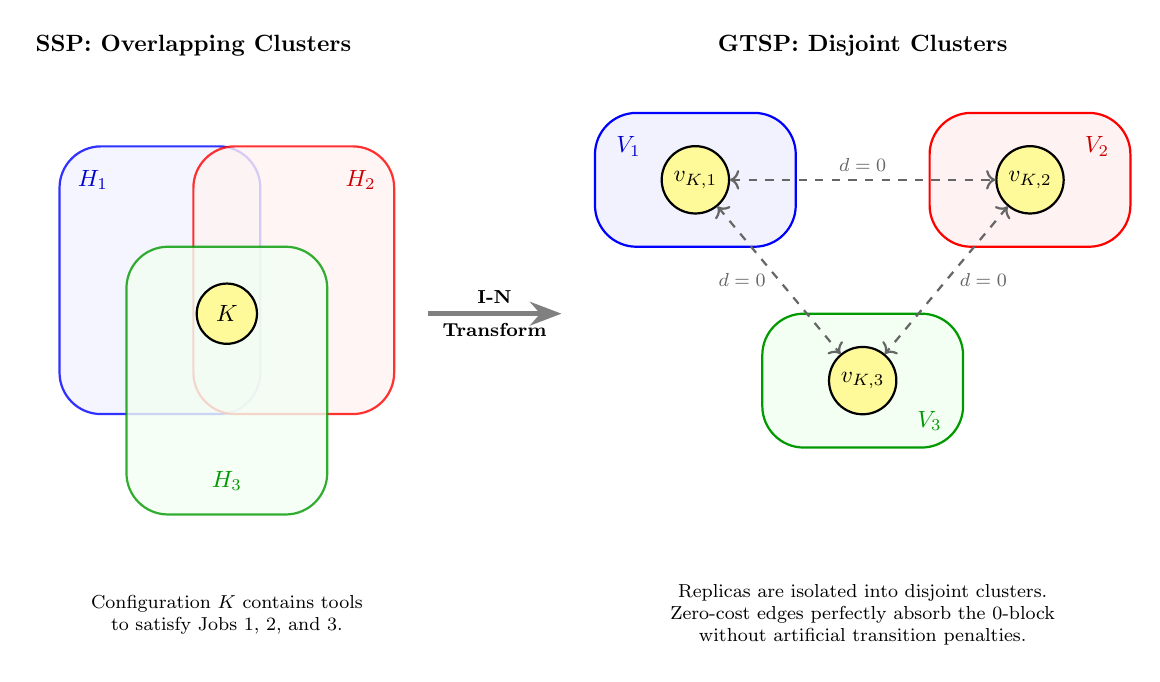
\begin{tikzpicture}[scale=0.85, every node/.style={transform shape}]
		
		% SSP Side
		\node[font=\bfseries] at (2, 5.5) {SSP: Overlapping Clusters};
		
		\draw[thick, blue, fill=blue!5, rounded corners=15pt, opacity=0.8] (0, 0) rectangle (3, 4);
		\node[blue!80!black, font=\bfseries] at (0.5, 3.5) {$H_{1}$};
		
		\draw[thick, red, fill=red!5, rounded corners=15pt, opacity=0.8] (2, 0) rectangle (5, 4);
		\node[red!80!black, font=\bfseries] at (4.5, 3.5) {$H_{2}$};
		
		\draw[thick, green!60!black, fill=green!5, rounded corners=15pt, opacity=0.8] (1, -1.5) rectangle (4, 2.5);
		\node[green!60!black, font=\bfseries] at (2.5, -1) {$H_{3}$};
		
		\node[draw, circle, fill=yellow!40, thick, minimum size=0.9cm] (K) at (2.5, 1.5) {$K$};
		
		\node[align=center, font=\footnotesize, text width=4.5cm] at (2.5, -3) {Configuration $K$ contains tools \\ to satisfy Jobs 1, 2, and 3.};
		
		% Arrow
		\draw[-{Stealth[length=4mm]}, line width=2pt, gray] (5.5, 1.5) -- (7.5, 1.5) 
		node[midway, above, font=\footnotesize\bfseries, text=black] {I-N} 
		node[midway, below, font=\footnotesize\bfseries, text=black] {Transform};
		
		% GTSP Side
		\node[font=\bfseries] at (12, 5.5) {GTSP: Disjoint Clusters};
		
		\draw[thick, blue, fill=blue!5, rounded corners=15pt] (8, 2.5) rectangle (11, 4.5);
		\node[blue!80!black, font=\bfseries] at (8.5, 4) {$V_{1}$};
		\node[draw, circle, fill=yellow!40, thick, minimum size=0.8cm] (v1) at (9.5, 3.5) {$v_{K, 1}$};
		
		\draw[thick, red, fill=red!5, rounded corners=15pt] (13, 2.5) rectangle (16, 4.5);
		\node[red!80!black, font=\bfseries] at (15.5, 4) {$V_{2}$};
		\node[draw, circle, fill=yellow!40, thick, minimum size=0.8cm] (v2) at (14.5, 3.5) {$v_{K, 2}$};
		
		\draw[thick, green!60!black, fill=green!5, rounded corners=15pt] (10.5, -0.5) rectangle (13.5, 1.5);
		\node[green!60!black, font=\bfseries] at (13, -0.1) {$V_{3}$};
		\node[draw, circle, fill=yellow!40, thick, minimum size=0.8cm] (v3) at (12, 0.5) {$v_{K, 3}$};
		
		% Zero Cost Edges
		\draw[<->, thick, dashed, gray!80!black] (v1) -- (v2) node[midway, above, font=\footnotesize\bfseries] {$d = 0$};
		\draw[<->, thick, dashed, gray!80!black] (v1) -- (v3) node[midway, left, font=\footnotesize\bfseries, xshift=-2pt] {$d = 0$};
		\draw[<->, thick, dashed, gray!80!black] (v2) -- (v3) node[midway, right, font=\footnotesize\bfseries, xshift=2pt] {$d = 0$};
		
		\node[align=center, font=\footnotesize, text width=6cm] at (12, -3) {Replicas are isolated into disjoint clusters. \\ Zero-cost edges perfectly absorb the 0-block \\ without artificial transition penalties.};
		
	\end{tikzpicture}
	\caption{Forward Mapping (SSP $\rightarrow$ GTSP). A single configuration $K$ covering three jobs is duplicated into mutually exclusive replicas connected by zero-cost edges, strictly preserving the optimal KTNS retention logic.}
	\label{fig:forward_mapping}
\end{figure}

\subsection{Reduction 2: GTSP to SSP (Reverse Mapping)}

To prove that the SSP is a strictly harder generalization, we must demonstrate that any arbitrary GTSP instance can be polynomially reduced to an SSP instance under a strict \textit{Disjointness Condition}. 

\textbf{The Construction:} Given an arbitrary GTSP instance $\mathcal{I}_{GTSP} = \langle V, E, d, \{V_k\}_{k \in K} \rangle$, we construct an SSP instance $\mathcal{I}_{SSP}$ as follows:
\begin{enumerate}
	\item \textbf{Jobs and Capacity:} Let the set of jobs $J = K = \{1, 2, \dots, k\}$. Set the magazine capacity $C = \max_{p=1}^k |V_p|$.
	\item \textbf{Tool Padding:} Let every vertex $v \in V$ become a unique tool. To prevent any single configuration of size $C$ from inadvertently covering multiple smaller clusters, we must enforce uniform tool requirements. For each cluster $V_p$, we generate a set of distinct dummy tools $D_p$ such that $|V_p \cup D_p| = C$. 
	\item \textbf{Tool Set:} The complete tool repository is $T = V \cup (\bigcup_{p=1}^k D_p)$.
	\item \textbf{Job Requirements:} For each job $p \in J$, define its tool requirement as $T_p = V_p \cup D_p$.
\end{enumerate}

\textbf{Proof of Correspondence:} In the original GTSP, clusters are mutually exclusive ($V_p \cap V_q = \emptyset$). Because our dummy tools $D_p$ are generated uniquely for each job, the padded tool requirements in our constructed SSP satisfy strict mutual exclusivity: $T_p \cap T_q = \emptyset$ for all $p \neq q$. 

Consequently, the union of any two distinct job requirements strictly requires $2C$ tools:
\begin{equation}
	|T_p \cup T_q| = |T_p| + |T_q| = 2C > C \quad \forall p \neq q
\end{equation}
Under this rigorous Disjointness Condition, no valid tool configuration $K$ (which is strictly bounded by $|K| \le C$) can possibly contain the tools to process more than one job. This enforces $H_p \cap H_q = \emptyset$ for all $p \neq q$. The configuration clusters in the SSP are structurally forced to be disjoint, collapsing the SSP back into a standard GTSP. 

\textbf{Computational Complexity:} The number of jobs $|J| = k$, the capacity $C \le |V|$, and the total number of tools $|T| \le k \cdot |V|$. This reverse transformation is bounded by $\mathcal{O}(k \cdot |V|)$, which is strictly \textbf{polynomial}. 

\begin{figure}[h!]
	\centering
	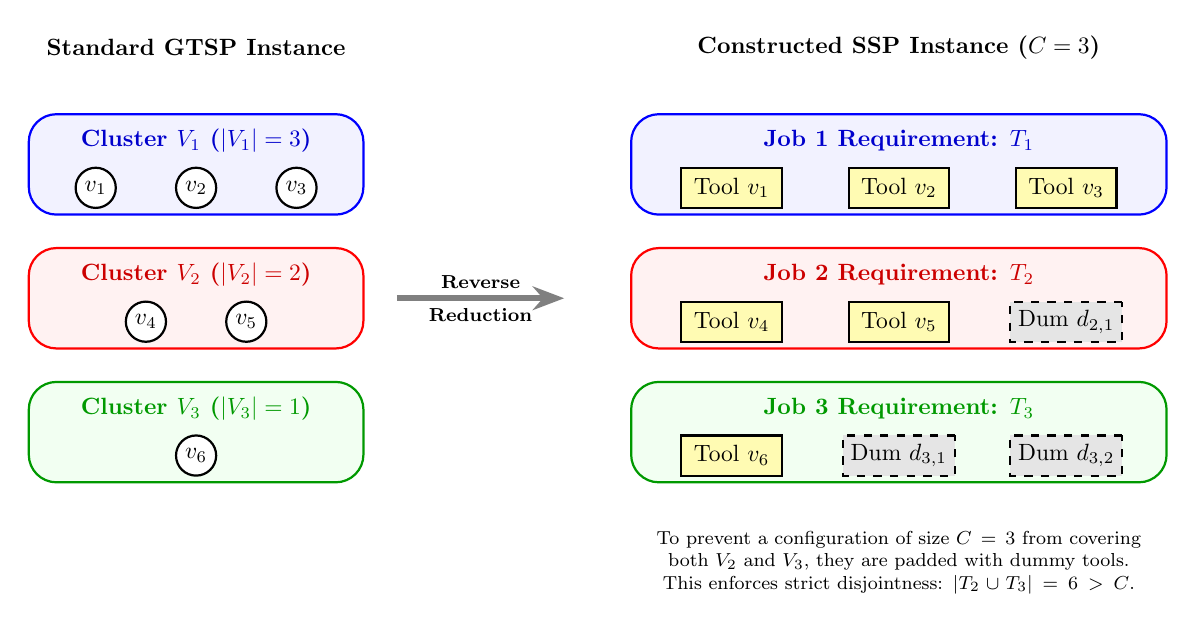
\begin{tikzpicture}[scale=0.85, every node/.style={transform shape}]
		
		% GTSP Side
		\node[font=\bfseries] at (2, 5.5) {Standard GTSP Instance};
		
		\draw[thick, blue, fill=blue!5, rounded corners=10pt] (-0.5, 3) rectangle (4.5, 4.5);
		\node[blue!80!black, font=\bfseries] at (2, 4.1) {Cluster $V_1$ ($|V_1| = 3$)};
		\node[draw, circle, fill=white, thick, minimum size=0.6cm, inner sep=1pt] (v1) at (0.5, 3.4) {$v_1$};
		\node[draw, circle, fill=white, thick, minimum size=0.6cm, inner sep=1pt] (v2) at (2, 3.4) {$v_2$};
		\node[draw, circle, fill=white, thick, minimum size=0.6cm, inner sep=1pt] (v3) at (3.5, 3.4) {$v_3$};
		
		\draw[thick, red, fill=red!5, rounded corners=10pt] (-0.5, 1) rectangle (4.5, 2.5);
		\node[red!80!black, font=\bfseries] at (2, 2.1) {Cluster $V_2$ ($|V_2| = 2$)};
		\node[draw, circle, fill=white, thick, minimum size=0.6cm, inner sep=1pt] (v4) at (1.25, 1.4) {$v_4$};
		\node[draw, circle, fill=white, thick, minimum size=0.6cm, inner sep=1pt] (v5) at (2.75, 1.4) {$v_5$};
		
		\draw[thick, green!60!black, fill=green!5, rounded corners=10pt] (-0.5, -1) rectangle (4.5, 0.5);
		\node[green!60!black, font=\bfseries] at (2, 0.1) {Cluster $V_3$ ($|V_3| = 1$)};
		\node[draw, circle, fill=white, thick, minimum size=0.6cm, inner sep=1pt] (v6) at (2, -0.6) {$v_6$};
		
		% Arrow
		\draw[-{Stealth[length=4mm]}, line width=2pt, gray] (5, 1.75) -- (7.5, 1.75) 
		node[midway, above, font=\footnotesize\bfseries, text=black] {Reverse} 
		node[midway, below, font=\footnotesize\bfseries, text=black] {Reduction};
		
		% SSP Side
		\node[font=\bfseries] at (12.5, 5.5) {Constructed SSP Instance ($C=3$)};
		
		\draw[thick, blue, fill=blue!5, rounded corners=10pt] (8.5, 3) rectangle (16.5, 4.5);
		\node[blue!80!black, font=\bfseries] at (12.5, 4.1) {Job 1 Requirement: $T_1$};
		\node[draw, rectangle, fill=yellow!30, thick, minimum height=0.6cm, minimum width=1.5cm] (t1) at (10, 3.4) {Tool $v_1$};
		\node[draw, rectangle, fill=yellow!30, thick, minimum height=0.6cm, minimum width=1.5cm] (t2) at (12.5, 3.4) {Tool $v_2$};
		\node[draw, rectangle, fill=yellow!30, thick, minimum height=0.6cm, minimum width=1.5cm] (t3) at (15, 3.4) {Tool $v_3$};
		
		\draw[thick, red, fill=red!5, rounded corners=10pt] (8.5, 1) rectangle (16.5, 2.5);
		\node[red!80!black, font=\bfseries] at (12.5, 2.1) {Job 2 Requirement: $T_2$};
		\node[draw, rectangle, fill=yellow!30, thick, minimum height=0.6cm, minimum width=1.5cm] (t4) at (10, 1.4) {Tool $v_4$};
		\node[draw, rectangle, fill=yellow!30, thick, minimum height=0.6cm, minimum width=1.5cm] (t5) at (12.5, 1.4) {Tool $v_5$};
		\node[draw, rectangle, fill=gray!20, dashed, thick, minimum height=0.6cm, minimum width=1.5cm] (d21) at (15, 1.4) {Dum $d_{2,1}$};
		
		\draw[thick, green!60!black, fill=green!5, rounded corners=10pt] (8.5, -1) rectangle (16.5, 0.5);
		\node[green!60!black, font=\bfseries] at (12.5, 0.1) {Job 3 Requirement: $T_3$};
		\node[draw, rectangle, fill=yellow!30, thick, minimum height=0.6cm, minimum width=1.5cm] (t6) at (10, -0.6) {Tool $v_6$};
		\node[draw, rectangle, fill=gray!20, dashed, thick, minimum height=0.6cm, minimum width=1.5cm] (d31) at (12.5, -0.6) {Dum $d_{3,1}$};
		\node[draw, rectangle, fill=gray!20, dashed, thick, minimum height=0.6cm, minimum width=1.5cm] (d32) at (15, -0.6) {Dum $d_{3,2}$};
		
		\node[align=center, font=\footnotesize, text width=8cm] at (12.5, -2.2) {To prevent a configuration of size $C=3$ from covering both $V_2$ and $V_3$, they are padded with dummy tools. \\ This enforces strict disjointness: $|T_2 \cup T_3| = 6 > C$.};
		
	\end{tikzpicture}
	\caption{Reverse Mapping (GTSP $\rightarrow$ SSP). Dummy tools enforce the Disjointness Condition, ensuring that no single valid tool configuration can cover multiple jobs, collapsing the SSP back into a GTSP.}
	\label{fig:reverse_reduction}
\end{figure}

\subsection{Algorithmic Implications of the Complexity Space}

Because the reverse reduction is polynomial while the forward reduction is exponential, the complete configuration graph cannot always be instantiated in memory. This inherent complexity difference dictates a bifurcated solution methodology (illustrated in Figure \ref{fig:complexity_flowchart}). 

For smaller instances where the capacity $C$ is restrictive, the entire GTSP graph can be generated, allowing polynomial transformations \parencite{Noon1993} to convert the problem into an Asymmetric TSP solvable by highly optimized routing heuristics. However, for massive instances where $\binom{|T|}{C}$ triggers out-of-memory failures, exactness requires dynamic node generation via Branch-and-Price, utilizing advanced learning strategies to navigate the exponential state space.

\begin{figure}[h!]
	\centering
	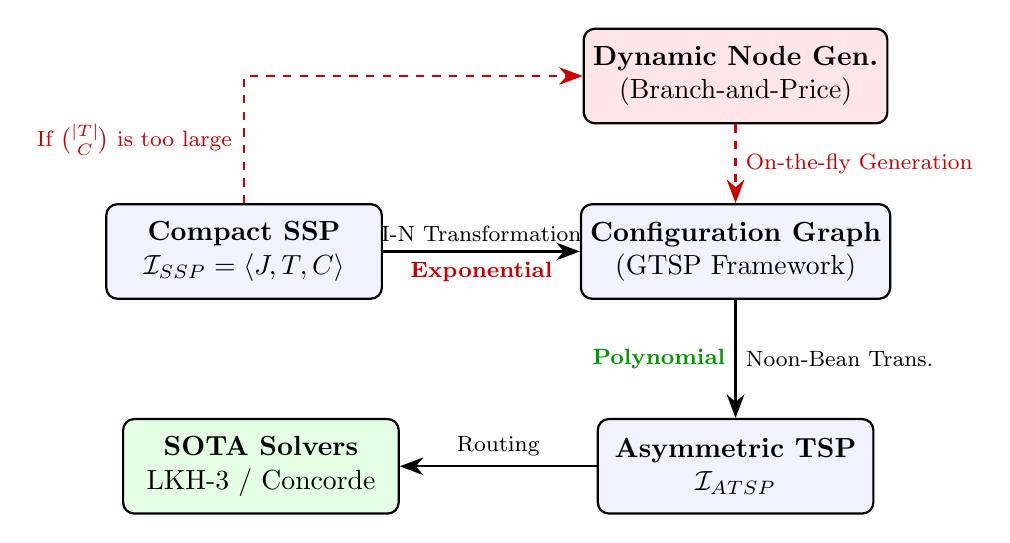
\begin{tikzpicture}[
		node distance=1.5cm and 2.5cm,
		box/.style={draw, rectangle, rounded corners, minimum width=3.5cm, minimum height=1.2cm, align=center, fill=blue!5, thick},
		arrow/.style={-{Stealth[length=3mm]}, thick}
		]
		
		% Nodes
		\node[box] (ssp) {\textbf{Compact SSP} \\ $\mathcal{I}_{SSP} = \langle J, T, C \rangle$};
		
		\node[box, right=of ssp] (gtsp) {\textbf{Configuration Graph} \\ (GTSP Framework)};
		
		\node[box, below=of gtsp] (atsp) {\textbf{Asymmetric TSP} \\ $\mathcal{I}_{ATSP}$};
		
		\node[box, fill=green!10, left=of atsp] (solvers) {\textbf{SOTA Solvers} \\ LKH-3 / Concorde};
		
		\node[box, fill=red!10, above=of gtsp, yshift=-0.5cm] (bp) {\textbf{Dynamic Node Gen.} \\ (Branch-and-Price)};
		
		% Arrows
		\draw[arrow] (ssp) -- node[above, font=\footnotesize] {I-N Transformation} node[below, font=\footnotesize\bfseries, text=red!80!black] {Exponential} (gtsp);
		
		\draw[arrow] (gtsp) -- node[right, font=\footnotesize] {Noon-Bean Trans.} node[left, font=\footnotesize\bfseries, text=green!60!black] {Polynomial} (atsp);
		
		\draw[arrow] (atsp) -- node[above, font=\footnotesize] {Routing} (solvers);
		
		\draw[arrow, dashed, red!80!black] (ssp) |- node[near start, left, font=\footnotesize, text width=2.5cm] {If $\binom{|T|}{C}$ is too large} (bp);
		\draw[arrow, dashed, red!80!black] (bp) -- node[right, font=\footnotesize] {On-the-fly Generation} (gtsp);
		
	\end{tikzpicture}
	\caption{The complexity space of solving the SSP. Tractable instances can be reduced to ATSP and solved via highly optimized routing heuristics, while massive instances bypass the exponential bottleneck via dynamic node generation in a Branch-and-Price framework.}
	\label{fig:complexity_flowchart}
\end{figure}

	
	\section{Exact Routing for Tractable Instances}
	
	For small-to-medium manufacturing environments, the total number of tools $|T|$ and the magazine capacity $C$ restrict the configuration space $\binom{|T|}{C}$ to a computationally manageable size. Under these conditions, the theoretical equivalence established in Section 3 allows us to entirely bypass the branch-and-bound bottlenecks of generic Integer Linear Programming (ILP) solvers like CPLEX or Gurobi.
	
	\subsection{The Noon-Bean Transformation}
	When the configuration space is tractable, the complete GTSP graph $G = (V, E)$ and its mutually exclusive clusters $\{V_j\}_{j \in J}$ can be explicitly instantiated in memory. Once instantiated, we apply the Noon-Bean transformation \parencite{Noon1993}. This rigorous graph transformation modifies the edge weights to compel any optimal routing algorithm to visit exactly one node per cluster before moving to the next.
	
	Consequently, the transformation collapses the generalized problem with overlapping configurations into a standard Asymmetric Traveling Salesman Problem (ATSP) over a directed graph. The resulting ATSP perfectly encodes the 0-block tool switching mechanics without the sequence-based symmetry that paralyzes compact models.
	
	\subsection{LKH-3 and Concorde}
	The reduction to an ATSP unlocks the application of the most powerful routing engines developed in the operations research community. The transformed graph can be fed directly into the Lin-Kernighan-Helsgaun (LKH-3) algorithm \parencite{Helsgaun2015}. LKH-3 utilizes highly advanced $k$-opt sequential exchanges and minimum spanning tree approximations to find optimal or near-optimal tours for asymmetric instances in fractions of a second \parencite{Helsgaun2015}. For environments requiring a mathematically proven global optimum, the ATSP can be solved using exact solvers such as Concorde \parencite{Applegate2006}. 
	
	This pathway demonstrates the immediate practical superiority of the non-compact formulation: tractable SSP instances can be translated directly into the domain of pure routing, solving in seconds what traditional compact models fail to solve in hours.
	
	
	\section{Dynamic Node Generation and the True Pricing Bottleneck}
	
	While the reduction to ATSP is definitive for small instances, it faces a hard mathematical limit in large-scale industrial settings. As the tool repository $m$ and magazine capacity $C$ grow, the number of valid configurations $\binom{m}{C}$ explodes exponentially. Generating the complete graph triggers severe out-of-memory failures. To maintain exactness without explicitly instantiating $V$, the problem must be solved dynamically using a Branch-and-Price (B\&P) framework \parencite{Barnhart1998}.
	
	\subsection{The Restricted Master Problem}
	In the B\&P framework, the algorithm initializes a \textit{Restricted Master Problem} (RMP) containing only a tiny, feasible subset of configuration nodes $V' \subset V$. The linear relaxation of the RMP is solved to obtain dual variables associated with both the job-covering constraints and the flow-conservation (routing) constraints.
	
	To prove global optimality or find improving configurations, these dual variables are passed to a Pricing Subproblem (PSP) oracle. The oracle's task is to identify a new configuration node $v \notin V'$ that possesses a negative reduced cost, meaning its addition to the RMP will improve the objective bound. 
	
	\subsection{The Complexity of the SSP Pricing Oracle}
	It is critical to distinguish the pricing complexity of the Tool Switching Problem (SSP) from that of the simpler Job Grouping Problem (JGP). In the JGP, the objective is purely a Set Covering task; the processing order of the configurations does not matter. Consequently, the JGP pricing oracle only needs to maximize the sum of the covering duals subject to the magazine capacity, a task formally equivalent to the Set Union Knapsack Problem (SUKP) \parencite{Crama1994}.
	
	However, the non-compact SSP formulation is a simultaneous covering \textit{and sequencing} problem. Because it maps to the GTSP, the cost of a configuration heavily depends on the transition edge weights $d(u,v)$ required to travel to and from that configuration in the sequence. Therefore, the reduced cost of a new configuration node in the SSP is not just a function of its internal tools (the knapsack component); it is an explicit function of its optimal insertion point in the current routing sequence, evaluated against the routing dual variables.
	
	To generate a new node with a negative reduced cost, the exact SSP pricing oracle must simultaneously determine the optimal subset of tools to fill the capacity $C$ \textit{and} compute the shortest transition paths from the existing nodes in the RMP. This creates an astronomically complex, strongly NP-hard pricing oracle. Evaluating this exact oracle at every single iteration of the column generation loop is computationally paralyzing. Thus, while the B\&P architecture provides a mathematically exact framework for large instances, the complexity of the routing-based pricing oracle remains the ultimate bottleneck to scalability.
	
	\section{Machine Learning for Dynamic Node Generation}
	
	Because the exact pricing oracle must simultaneously solve a Set Covering problem for the tools and evaluate routing transitions for the sequence, executing it exactly at every iteration of the Branch-and-Price (B\&P) tree is computationally paralyzing. To bridge this gap, we propose augmenting the configuration-based SSP formulation with the latest advancements in Machine Learning (ML). Rather than solving the exact oracle, ML models can be trained to heuristically predict and generate the most promising configuration nodes, falling back to the exact pricing algorithm only when necessary \parencite{Karimi2022}.
	
	\subsection{Bipartite State Representation}
	To train an Artificial Intelligence agent to guide the node generation process, the operational state of the Restricted Master Problem (RMP) must be mathematically encoded. Recent literature highlights that an RMP naturally forms a bipartite graph: one set of vertices represents the constraints (the required jobs), while the other represents the active columns (the tool configurations currently in the ATSP basis) \parencite{Chi2022}. 
	
	By mapping the edges to indicate which configurations cover which jobs, the entire state of the SSP sequence can be processed by Graph Neural Networks (GNNs). These networks extract high-dimensional latent embeddings that capture the complex interrelations between unsatisfied jobs, current tool magazine states, and existing sequence transitions, allowing the AI to effectively "read" the optimization landscape \parencite{Chi2022}.
	
	\subsection{Reinforcement Learning for Node Selection}
	Traditional Column Generation algorithms employ a myopic greedy strategy, searching for a single column with the most negative reduced cost. However, frameworks such as RLCG demonstrate that column (or node) selection is fundamentally a sequential Markov Decision Process (MDP) \parencite{Chi2022}. 
	
	By utilizing Deep Reinforcement Learning (DRL), an agent can evaluate the bipartite GNN state and select nodes that maximize long-term rewards---specifically, minimizing the total number of pricing iterations required for the ATSP relaxation to converge. Furthermore, to combat degeneracy and accelerate routing optimization, the DRL agent can execute a \textit{Multiple-Node Selection Strategy}. Instead of adding a single node, the agent selects a diverse, non-correlated batch of configurations to inject into the graph simultaneously, providing the routing solver with a richer subspace to optimize \parencite{Yuan2023}.
	
	\subsection{Preserving the Exactness Guarantee}
	The paramount advantage of this ML-augmented pathway is that it maintains the mathematical exactness of the Branch-and-Price tree. The GNN and DRL agents act purely as a rapid heuristic filter for the Pricing Subproblem. They instantly identify and inject highly promising nodes into the ATSP graph. Only if the ML agent fails to find a configuration with a negative reduced cost does the algorithm trigger the exact pricing oracle to prove optimality \parencite{Vaclavik2018}. Thus, the global optimality guarantee of the B\&P framework remains intact, while the average computational time is drastically reduced.
	
	\section{Conclusion}
	
	The Job Sequencing and Tool Switching Problem (SSP) is a fundamental optimization challenge in flexible manufacturing. This report has demonstrated that traditional compact integer programming formulations suffer from crippling 0-block symmetries and weak linear relaxations. By adopting a non-compact, configuration-based formulation, we mathematically eradicated these sequence-based symmetries and established a rigorous two-way equivalence between the SSP and the Generalized Traveling Salesman Problem (GTSP).
	
	This theoretical bridge unlocks two distinct, advanced algorithmic pathways based on the complexity space of the instance. For tractable manufacturing environments, the configuration graph can be fully instantiated and mapped via the Noon-Bean transformation to an Asymmetric TSP. This allows for exact or near-exact solutions in seconds using state-of-the-art routing engines like LKH-3 and Concorde. For massive industrial instances where the graph size explodes exponentially, the formulation naturally decomposes into a Branch-and-Price framework. Because the pricing oracle must handle both tool capacities and routing transitions, it is extremely complex. However, by leveraging the bipartite structure of the Restricted Master Problem, we propose that integrating Graph Neural Networks and Deep Reinforcement Learning can successfully bypass this pricing bottleneck. Ultimately, the configuration-based formulation provides a robust mathematical foundation for hybridizing classical Operations Research with modern Artificial Intelligence, charting a definitive path toward solving the SSP at an industrial scale.
	
	\printbibliography
	
\end{document}